\documentclass[12pt,a4paper,UTF8]{article}
% \usepackage{ctex} % Chinese support
\usepackage{graphicx} % Insert images
\usepackage{listings} % Print source code
\usepackage{color} % Color support
\usepackage{booktabs} % Professional table support
\usepackage{pdflscape} % Landscape pages support in PDF
\usepackage{hyperref} % Hypertext links support for cross-referencing

% Customize hyperref format (it's set to no special format here)
\hypersetup{hidelinks}

% Declare directories to search for graphics files for graphicx
\graphicspath{{figures/}{logo/}}

% Define source code style for listings
\lstdefinestyle{python}{
  language=Python,
  basicstyle=\ttfamily\footnotesize,
  keywordstyle=\bfseries\color[rgb]{0, 0, 1},
  identifierstyle=\color[rgb]{0.5, 0.3, 0.1},
  stringstyle=\color[rgb]{0.6, 0.1, 0.1},
  commentstyle=\itshape\color[rgb]{0.05, 0.5, 0.05},
  backgroundcolor=\color[gray]{0.95},
  numbers=left,
  numbersep=5pt,
  numberstyle=\color[gray]{0.6},
  breaklines=true
}

% Define new command for title page
\newcommand{\reporttitle}[2]{
  \LARGE\textsf{#1}\quad\underline{\makebox[12em]{#2}}
}
\newcommand{\reportinfo}[2]{
  \large\makebox[4em]{\textsf{#1}}\quad\underline{\makebox[18em]{#2}}
}

% The document begins here
\begin{document}
\begin{titlepage}
  \centering
  \vspace*{\fill}
  
\includegraphics[height=144pt]{nju-logo}\\[48pt]
  {\huge\textsf{Lab Report}}\\[48pt]
  \reporttitle{Lab Name}{Reliable Communication}\\[72pt]

  \reportinfo{Course}{Computer Network}\\[8pt]
  \reportinfo{Major}{Computer Science and Technology}\\[8pt]
  \reportinfo{Id}{191220129}\\[8pt]
  \reportinfo{Name}{Shangyu.Xing}\\[8pt]
  \reportinfo{Email}{191220129@smail.nju.edu.cn}\\[8pt]
  \reportinfo{Date}{2021.05}\\
  \vspace*{\fill}
\end{titlepage}

\tableofcontents
\newpage

\section{Objective}
\begin{itemize}
	\item Learn reliable communication and how to implement it;
	\item learn to implement hardware logic using the Switchyard framework;
	\item learn to capture network package using wireshark.
\end{itemize}

\section{Requirements}
	This lab requires to implement a simplified network which achieves reliable communication. It has 3 main components:
\begin{itemize}
	\item MiddleBox:
	\subitem forward packets directly from one interface to another;
	\subitem drop packets according to dropRate.
	\item blastee: send a corresponding ack upon receiving a packet from blaster;
	\item blaster:
	\subitem send packets;
	\subitem receive acks and maintain a sender window;
	\subitem retransmit if timeout;
	\subitem do statistics.
\end{itemize}

\section{Procedure}
I completed all the tasks as required.
In this section, I will explain how I did my work in detail.

\subsection{Packet Structure}
Before coming to the detailed implementation, I'd like to introduce my packet structure. A packet blaster send out or an ack blastee send out consists of 4 parts (or has 4 headers) -- Ethernet, IPv4, UDP and RawPacketContent. The differences are in RawPacketContent, as illustrated below:
\begin{figure}[htbp]
	\centering
	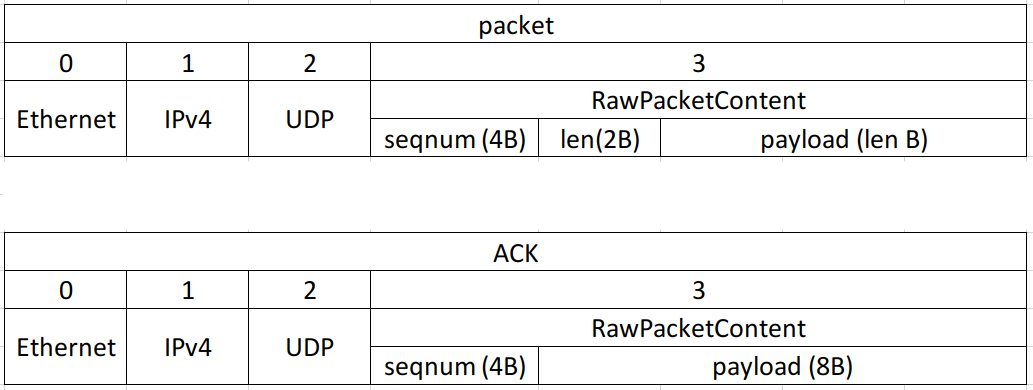
\includegraphics[width=\textwidth]{1}
	\caption{packet structure}
\end{figure}

\subsection{MiddleBox}
MiddleBox should do the following when receive a packet:
\begin{enumerate}
	\item Check where the packet comes from;
	\item if it is from blastee, forward it to blaster (only srcmac and dstmac should be modified);
	\item if it is from blaster, get a random value in [0,1] and drop the packet if it is below dropRate, otherwise forward it.
\end{enumerate}
Uncertain behavior introduced by random value means a painful debugging process. To make the result reproduceable, I manually set the random seed to 0.
\lstinputlisting[style=python]{1.py}

\subsection{Blastee}
Blastee sends an ack back when receiving a packet from blaster. According to packet structure, It should do the following:
\begin{enumerate}
	\item Create Ethernet, IPv4, UDP headers and fill in src and dst field;
	\item copy [0:4] byte from RawPacketContent of the received packet into ack's RawPacketContent (since it is sequence number);
	\item extract [4:6] byte as payload length;
	\item if it is larger than 8, copy the first 8 bytes of payload into ack's payload;
	\item if not, copy payload and pad to 8 bytes.
\end{enumerate}
\lstinputlisting[style=python]{2.py}

\subsection{Blaster}
The core part of blaster is how to implement the sender window. The most natural implementation is using an array storing all packets to be sent and two pointers indicating left and right edge of the window. However, that requires a huge amount of storage which is unacceptable on actual host. So I used a deque to represent the sender window -- move left edge equivalent to popleft and move right edge equivalent to appendright.
I created a class called Buffer to capsulize data and operation related to deque.
Here is the detailed implementation.

\subsubsection{create new packet}
New packets should be created before inserting into deque. We must maintain sequence number in the process.
\lstinputlisting[style=python]{3.py}

\subsubsection{handle ack packet}
When received an ack, extract sequence number and match that in the sender window. Then move left edge and right edge accordingly.
\lstinputlisting[style=python]{4.py}

\subsubsection{check timeout}
If blaster doesn't receive an ack in recvTimeout, it should check timeout of the sender window. If timeout it will retrainsmit.
\lstinputlisting[style=python]{5.py}

\section{Test \& Result}
I tested my code in mininet with dropRate = 0.4, num = 10 and the result is below (the capture file is saved in report/).
\begin{figure}[htbp]
	\centering
	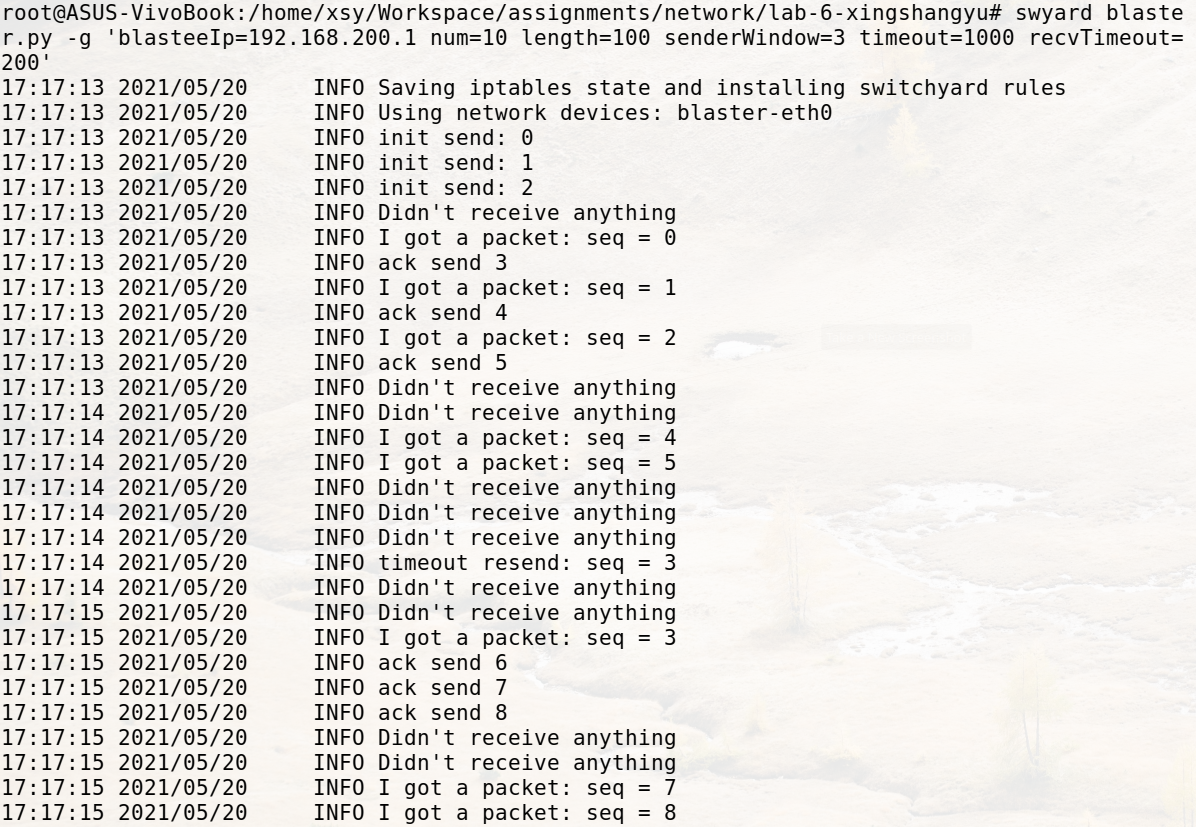
\includegraphics[width=\textwidth]{2}
	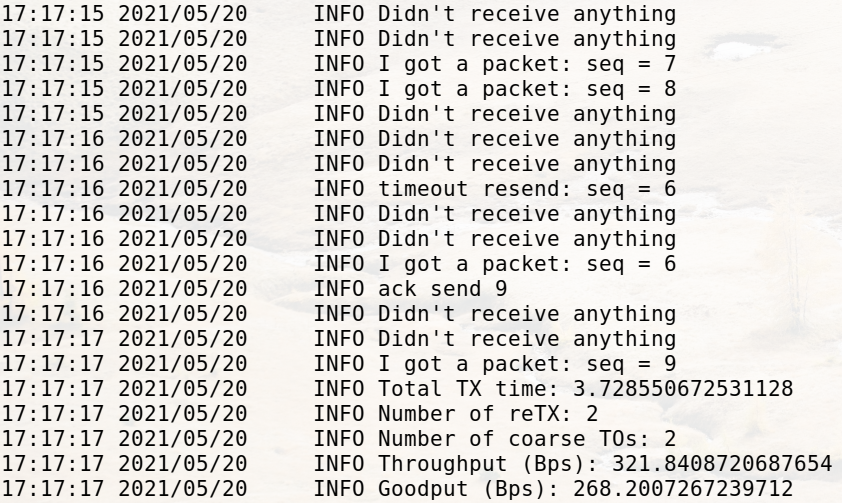
\includegraphics[width=0.7\textwidth]{3}
	\caption{blaster's log}
\end{figure}
\begin{figure}[htbp]
	\centering
	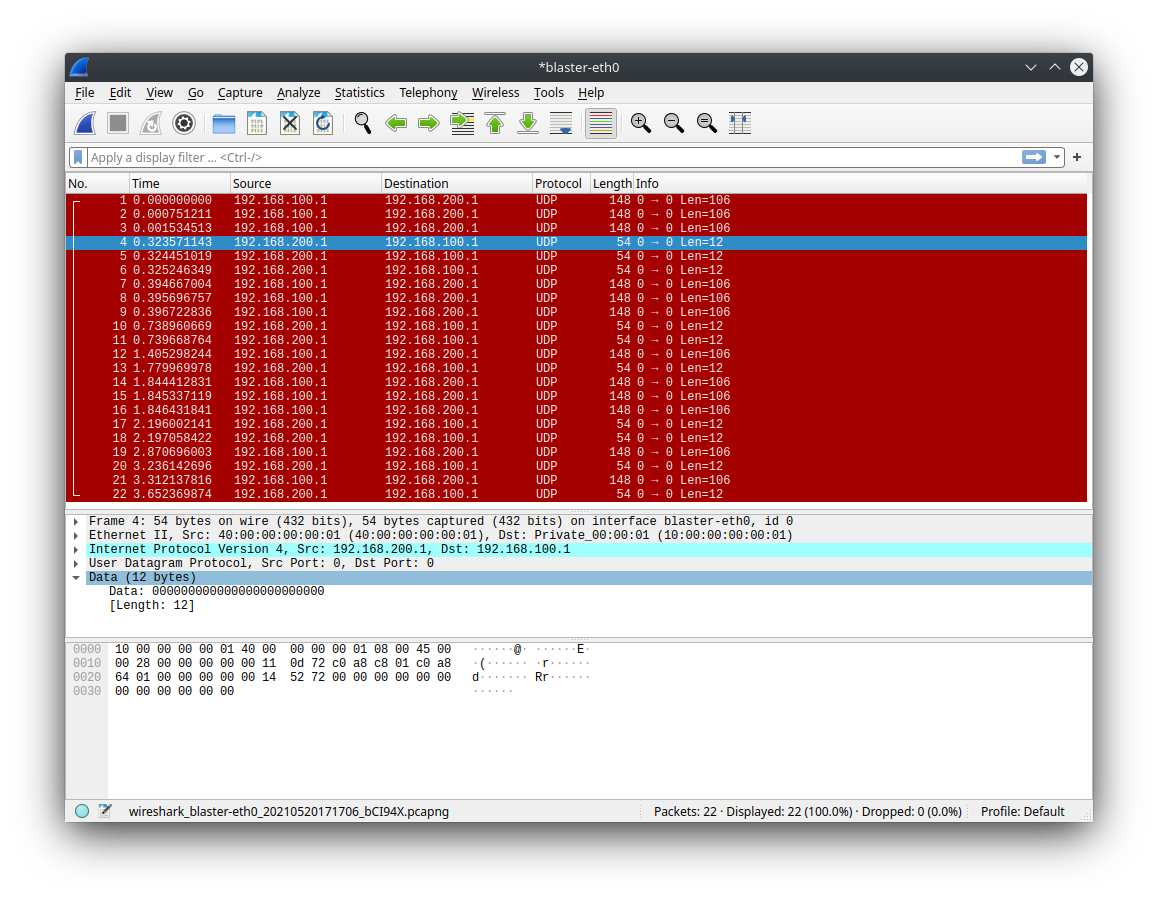
\includegraphics[width=\textwidth]{4}
	\caption{wireshark capture result}
\end{figure}
\newpage
We can learn from the log and capture result that:
\begin{itemize}
	\item in the 13s, blaster received 3 acks, so it moved the sender window and sent 3 new packets;
	\item in the 14s, blaster received acks for packet 4 and 5, but packet 3 timeout (dropped in middlebox), so it resent packet 3;
	\item the program ended when the last packet (packet 9) was acked.
\end{itemize}
The behavior of the network was the same as expected, so I have confidence that my program is correct. \\
Lastly, I present here the test result of the default parameters:
\begin{figure}[htbp]
	\centering
	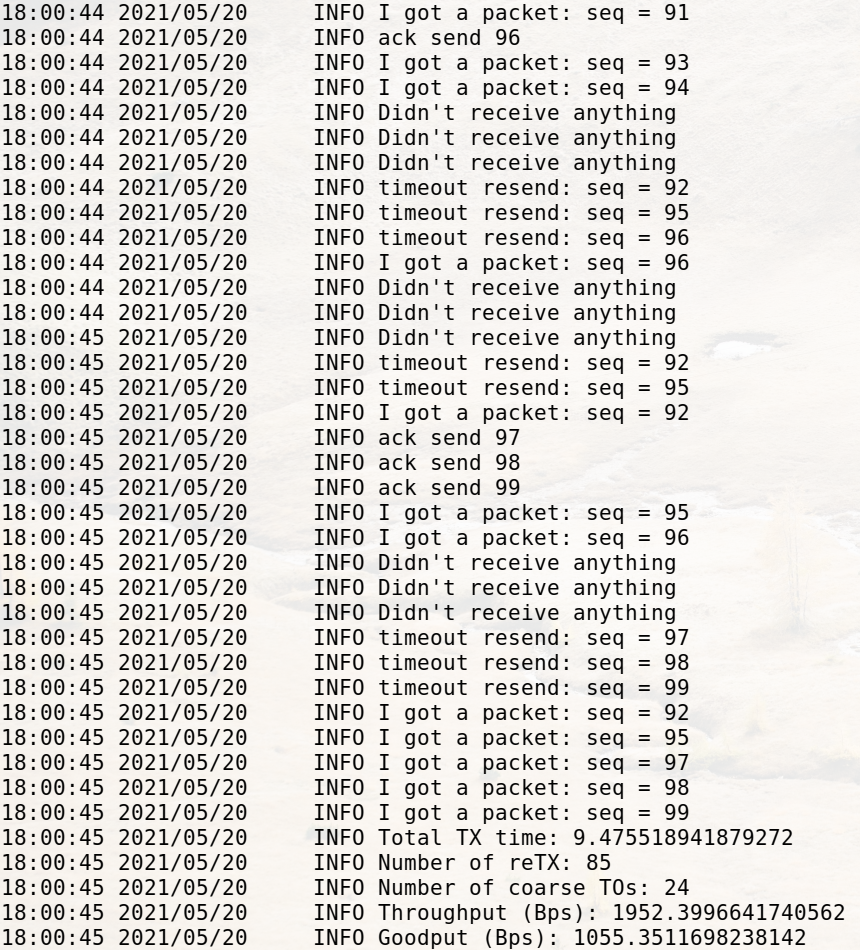
\includegraphics[width=\textwidth]{5}
	\caption{test result with default parameters}
\end{figure}

\newpage
\section{Summary}
\begin{itemize}
	\item Knowing how to effectively use debugging tools such as pdb will greatly enhance working efficiency;
	\item English reading and writing skills are important.
\end{itemize}

\end{document}